\documentclass[]{jsarticle}
\usepackage[dvipdfmx]{graphicx}
\usepackage{fancyvrb}
\usepackage{bm}
\usepackage{listings,jlisting} %日本語のコメントアウトをする場合jvlisting(もしくはjlisting)が必要
%ここからソースコードの表示に関する設定
\lstset{
  basicstyle={\ttfamily},
  identifierstyle={\small},
  commentstyle={\smallitshape},
  keywordstyle={\small\bfseries},
  ndkeywordstyle={\small},
  stringstyle={\small\ttfamily},
  frame={tb},
  breaklines=true,
  columns=[l]{fullflexible},
  numbers=left,
  xrightmargin=0zw,
  xleftmargin=3zw,
  numberstyle={\scriptsize},
  stepnumber=1,
  numbersep=1zw,
  lineskip=-0.5ex
}

\begin{document}
%
\section{課題I}
%
%
%
\subsection{課題I-1}
%
%
\subsubsection{GLEW}
GLEWとは,グラフィックスハードウェアの拡張機能を使用可能にするライブラリである.特にWindowsでは,もともとサポートしているOpenGLのバージョンが1.1のため,新しい機能を使用することができない.そのため,GLEWを用いてグラフィックスハードウェアが持つ全ての機能を使えるようにする.
%
%
%
\subsubsection{GLFW}
GLFWとは,デスクトップでのOpenGL,OpenGL ES,Vulkan開発用のオープンソースのマルチプラットフォームライブラリである.ウィンドウやコンテキストを作成し,入力を管理するためのシンプルなAPIを提供する.
%
%
\subsubsection{GLUI}
GLUIとは,ダイアログウィンドウで使用されるボタンやチェックボックスなどのコントロールをOpenGLで作成できるライブラリである.
%
%
\subsubsection{Vulkan}
Vukanとは,グラフィックスAPIのことで,直接GPUにアクセスできる構造によって,これまでのグラフィックスAPIに比べてより速い描画をすることが可能となる.
%
%
\subsubsection{OpenGL ES}
OpenGL ESとは,電化製品や車両などの組み込みおよびモバイルシステムで,高度な2D,3DグラフィックスをレンダリングするためのクロスプラットフォームAPIである.
%
%
\subsubsection{WebGL}
WebGLとは,ウェブブラウザ上でOpenGL ES相当の描画処理を行うことができる低レベルのAPIである.JavaScriptのAPIとして実装されているため,改めてプラグイン等をインストールすることなく実行できる.
%
%
%
\subsection{課題I-2}
\subsubsection{makeユーティリティ}
makeとは大規模プログラムのコンパイルを簡略化するツールである.makefileにファイルの関係を記述することで,各ファイルの更新を取得し,必要なものだけをコンパイルすることができる.以下のコマンドでmakefileを実行することができる.
\begin{lstlisting}[]
make
\end{lstlisting}

\subsubsection{grep}
grepとは,テキストファイルの中から正規表現と一致する行を検索し,出力するコマンドである.以下のコマンドでgrepを使用することができる.
\begin{lstlisting}[]
grep [オプション] [検索文字列(正規表現)] [ファイル名]
\end{lstlisting}

\subsubsection{touch}
touchとはファイルの最終更新日を変更するコマンドである.以下のコマンドでtouchを使用することができる.
\begin{lstlisting}[]
touch [オプション] ファイル1 ファイル2 …
\end{lstlisting}

\subsubsection{CMake}
CMakeとは,ソフトウェアをビルドやテスト,パッケージ化するために設計されたオープンソースのクロスプラットフォームツールである.プラットフォームやコンパイラに依存しないシンプルな設定ファイルを使用することでソフトウェアのコンパイルプロセスを制御し,makefileとワークスペースを生成するために使用される.

\subsubsection{Subversion}
Subversionとは,データの安全な避難所としての信頼性を特徴とするオープンソースの集中型バージョン管理システムである.個人から大規模なエンタープライズオペレーションまで,さまざまなユーザやプロジェクトのニーズをサポートすることができる.

\subsubsection{Git}
Gitとは,小規模なプロジェクトから大規模なプロジェクトまで,効率的に処理できるように設計されたオープンソースの分散型バージョン管理システムである.非常に高速なパフォーマンスを備えた小さなフットプリントを備えている.

\subsection{課題I-3}
C言語での変数は,その宣言を書く場所によって有効範囲(スコープ)が異なる.変数のスコープ外からは,その変数を参照することができない.一方,どの関数にも属さない場所で宣言された変数をグローバル変数と呼び,プログラム内のどこからでもアクセスが可能となる.
記憶域期間には自動記憶域期間と静的記憶域期間がある.自動記憶域期間を持つ変数はautoを使用して宣言される.この変数の記憶寿命は宣言した関数内に入った時から出る時までである.このように,関数内で宣言され,自動記憶域期間をもつ変数をローカル変数という.一方,staticを使用して宣言された変数は静的記憶域期間を持ち,記憶寿命はプログラムの開始から終了までとなる.このような変数をスタティック変数と呼ぶ.

\subsection{課題I-4}
星形正多角形を描き,回転させるプログラムの主要部をソースコード\ref{star}に示す.
\begin{lstlisting}[caption=星形正多角形の描画と回転,label=star]
void display() {
    glClear(GL_COLOR_BUFFER_BIT);
    glColor3d(1.0, 1.0, 1.0);

    dt = 2.0 * M_PI / NUM;
    theta = rotAng;
    
    for (i = 0; i < NUM; i++) {
        x[i] = cos(theta);
        y[i] = sin(theta);
        theta += dt;
    }

    for (i = 0; i < NUM; i++) {
        glBegin(GL_LINES);
        glVertex2d(x[i], y[i]);
        glVertex2d(x[(i + 2) % NUM], y[(i + 2) % NUM]);
        glEnd();
    }

    glFlush();
    rotAng += 3.0 * M_PI / 180.0;
}
\end{lstlisting}
定数NUMを変更することで,星型正多角形の角の数を変えることができる.

星型正多角形を描くには,全頂点において,2つ隣の頂点に線を引くことで描画することができる.そのため,あらかじめ線を引く頂点の座標を配列に格納し,GL\_LINESを用いることで線を引く.変数thetaをインクリメントすることで全頂点においてこの作業を行う.

このプログラムを使用して描画した星型正五角形と星型正六角形を図\ref{fig:5star},\ref{fig:6star}に示す.
\begin{figure}[htbp]
\begin{center}
\begin{minipage}[b]{0.45\textwidth}
  \begin{center}
    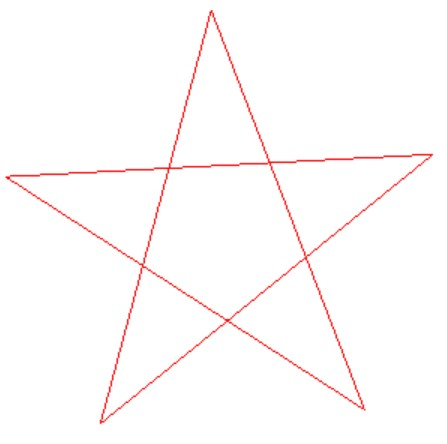
\includegraphics[width=4cm,keepaspectratio]{5star.jpg}
    \caption{星型正五角形}
    \label{fig:5star}
  \end{center}
\end{minipage}
\begin{minipage}[b]{0.45\textwidth}
  \begin{center}
    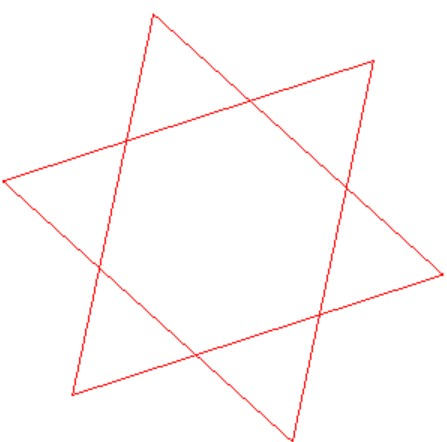
\includegraphics[width=4cm,keepaspectratio]{6star.jpg}
    \caption{星型正六角形}
    \label{fig:6star}
  \end{center}
\end{minipage}
\end{center}
\end{figure}
\subsection{課題I-5}
完全グラフを描き,回転させるプログラムの主要部をソースコード\ref{superstar}に示す.
\begin{lstlisting}[caption=完全グラフの描画と回転,label=superstar]
void display() {
    glClear(GL_COLOR_BUFFER_BIT);
    glColor3d(1.0, 1.0, 1.0);

    dt = 2.0 * M_PI / NUM;
    theta = rotAng;

    for (i = 0; i < NUM; i++) {
        x[i] = cos(theta);
        y[i] = sin(theta);
        theta += dt;
    }

    for (i = 0; i < NUM; i++) {
        for (j = i + 1; j < NUM; j++) {
            glBegin(GL_LINES);
            glVertex2d(x[i], y[i]);
            glVertex2d(x[j], y[j]);
            glEnd();
        }
    }

    glFlush();
    rotAng += 3.0 * M_PI / 180.0;
}
\end{lstlisting}
定数NUMを変更することで,完全グラフの角の数を変えることができる.

完全グラフを描くには,全頂点において,他の頂点全てに線を引くことで描画することができる.そのため,あらかじめ線を引く頂点の座標を配列に格納し,GL\_LINESを用いることで線を引く.その際,すでに線を引いてある2点間について,重ねて線を引かないように,15行目に書いてあるように,ループ数を減らしていく.変数thetaをインクリメントすることで全頂点においてこの作業を行う.

このプログラムを使用して描画した星型正五角形と星型正六角形を図\ref{fig:5p},\ref{fig:6p}に示す.
\begin{figure}[htbp]
\begin{center}
\begin{minipage}[b]{0.45\textwidth}
  \begin{center}
    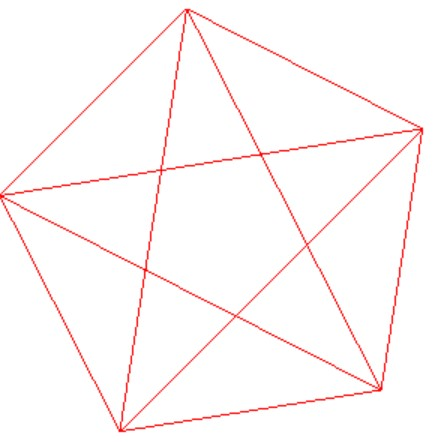
\includegraphics[width=4cm,keepaspectratio]{5p.jpg}
    \caption{5頂点完全グラフ}
    \label{fig:5p}
  \end{center}
\end{minipage}
\begin{minipage}[b]{0.45\textwidth}
  \begin{center}
    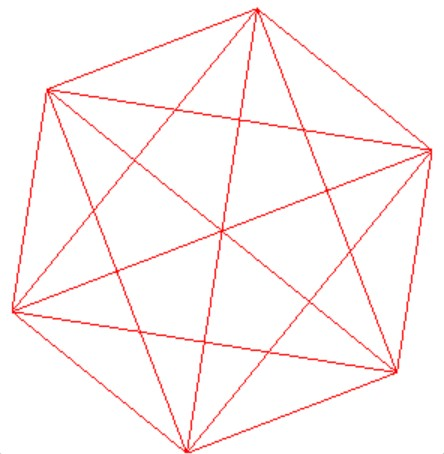
\includegraphics[width=4cm,keepaspectratio]{6p.jpg}
    \caption{6頂点完全グラフ}
    \label{fig:6p}
  \end{center}
\end{minipage}
\end{center}
\end{figure}

\subsection{課題I-6}
カージオイド,サイクロイド,4尖点の内サイクロイドを描画するプログラムの主要部を,それぞれソースコード\ref{cardioid},\ref{cycloid},\ref{hypocycloid}に示す.

\begin{lstlisting}[caption=カージオイドの描画,label=cardioid]
void display(void){
	glColor3d(0.0, 0.0, 1.0);
	glBegin(GL_LINE_STRIP);
	
	for (theta = 0; theta <= 2 * M_PI; theta += 2 * M_PI / 100) {
		x = cos(theta) * (1 + cos(theta));
		y = sin(theta) * (1 + cos(theta));
		glVertex2d(x, y);
	}
	
	glEnd();
	glFlush();
}
\end{lstlisting}

\begin{lstlisting}[caption=サイクロイドの描画,label=cycloid]
void display(void){
	glColor3d(0.0, 0.0, 1.0);
	glBegin(GL_LINE_STRIP);
	
	for (theta = 0; theta <= 2 * M_PI; theta += 2 * M_PI / 100) {
		x = theta - sin(theta);
		y = 1 - cos(theta);
		glVertex2d(x, y);
	}
	
	glEnd();
	glFlush();
}
\end{lstlisting}

\begin{lstlisting}[caption=4尖点の内サイクロイドの描画,label=hypocycloid]
void display(void){
	glColor3d(0.0, 0.0, 1.0);
	glBegin(GL_LINE_STRIP);
	
	for (theta = 0; theta <= 2 * M_PI; theta += 2 * M_PI / 100) {
		x = (cos(theta)) * (cos(theta)) * (cos(theta));
		y = (sin(theta)) * (sin(theta)) * (sin(theta));
		glVertex2d(x, y);
	}
	
	glEnd();
	glFlush();
}
\end{lstlisting}

$\theta$は0から$2\pi$まで変化させ,100点間を線で結んでいる.描画したグラフを図\ref{fig:cardioid},\ref{fig:hypocycloid},\ref{fig:cycloid}に示す.

\begin{figure}[htbp]
\begin{center}
\begin{minipage}[b]{0.45\textwidth}
  \begin{center}
    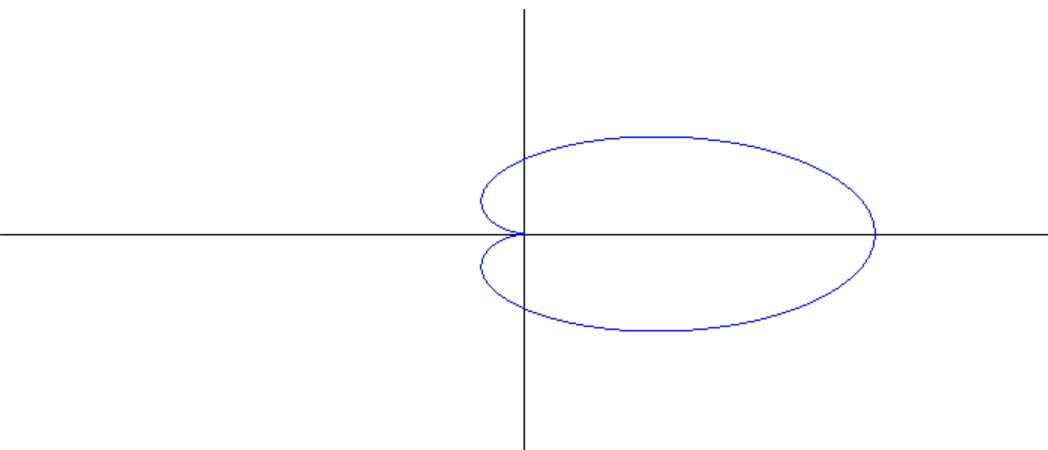
\includegraphics[width=6cm,keepaspectratio]{a.jpg}
    \caption{カージオイド}
    \label{fig:cardioid}
  \end{center}
\end{minipage}
\begin{minipage}[b]{0.45\textwidth}
  \begin{center}
    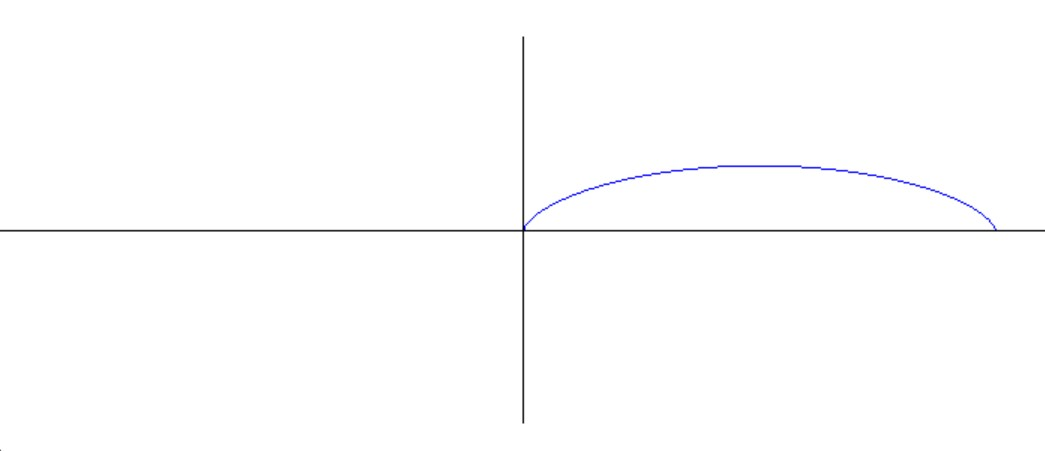
\includegraphics[width=6cm,keepaspectratio]{b.jpg}
    \caption{サイクロイド}
    \label{fig:hypocycloid}
  \end{center}
\end{minipage}
\end{center}
\end{figure}
\begin{figure}[htbp]
\begin{center}
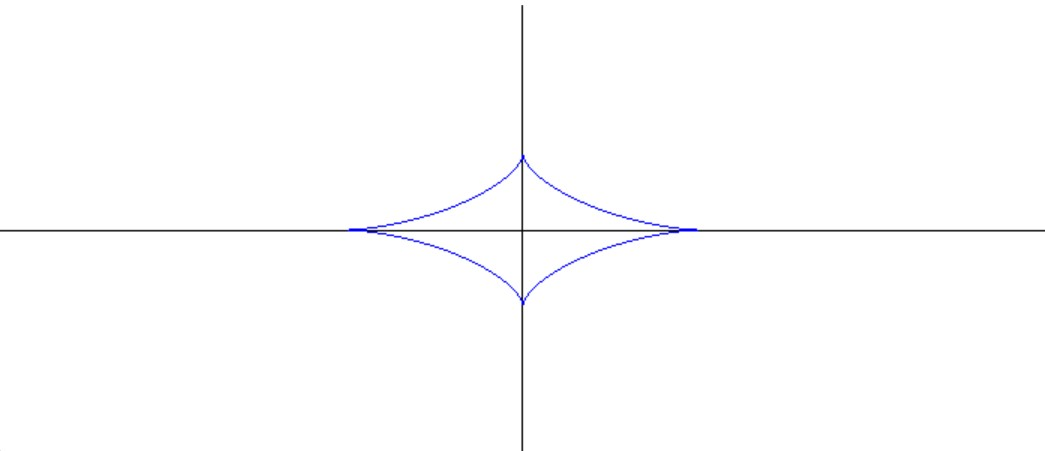
\includegraphics[height=3cm,keepaspectratio]{c.jpg}
    \caption{4尖点の内サイクロイド}
    \label{fig:cycloid}
\end{center}
\end{figure}

\section{課題II}
\subsection{課題II-1}
右手系の座標を考える.頂点$A$は$x$軸上の点だから$y$,$z$座標は0となり,$x$座標については,辺AGの長さから求められる.頂点$B$は$y$軸上の点だから$x$,$z$座標は0となり,$y$座標については,辺BGの長さから求められる.頂点$C$,$D$は,$y$-$z$平面の点だから$x$座標は0となる.また,$y$座標は辺GHの長さから求められ,$z$座標は,それぞれ辺CH,DHの長さから求められる.

正四面体の一辺の長さを$w$として各辺の長さを求める.図\ref{fig:bcd}に示すように,三角形の重心は中線を2:1に内分するため,辺BGの長さは$\frac{\sqrt{3}}{3}w$,辺GHの長さは$\frac{\sqrt{3}}{6}w$となる.図\ref{fig:bga}に示すように,$\triangle{\rm{BGA}}$に三平方の定理を適用すると,辺AGの長さは$\frac{\sqrt{6}}{3}w$となる.点$H$は辺CDの中点であるから,辺CH,辺DHは$\frac{w}{2}$となる.よって各頂点の座標は以下のようになる.
\begin{eqnarray*}
		&A&:(\frac{\sqrt{6}}{3}w, 0, 0) \\
		&B&:(0, \frac{\sqrt{3}}{3}w, 0)\\
		&C&:(0, -\frac{\sqrt{6}}{3}w, \frac{w}{2})\\
		&D&:(0, -\frac{\sqrt{6}}{3}w, -\frac{w}{2}) 
\end{eqnarray*}

\begin{figure}[htbp]
\begin{center}
\begin{minipage}[b]{0.45\textwidth}
  \begin{center}
    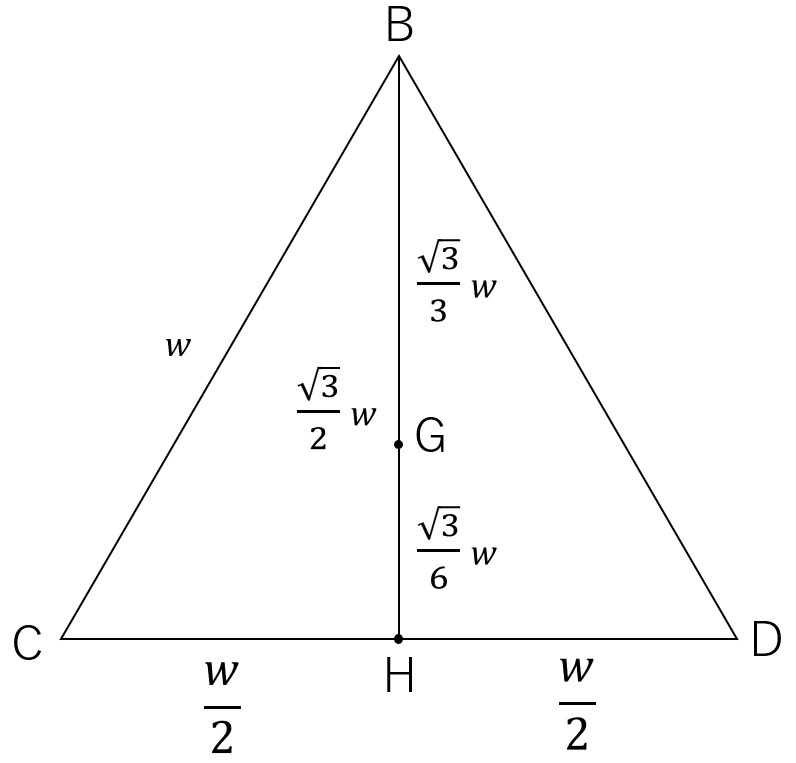
\includegraphics[width=6cm,keepaspectratio]{BCD.jpg}
    \caption{$\triangle{\rm{BCD}}$}
    \label{fig:bcd}
  \end{center}
\end{minipage}
\begin{minipage}[b]{0.45\textwidth}
  \begin{center}
    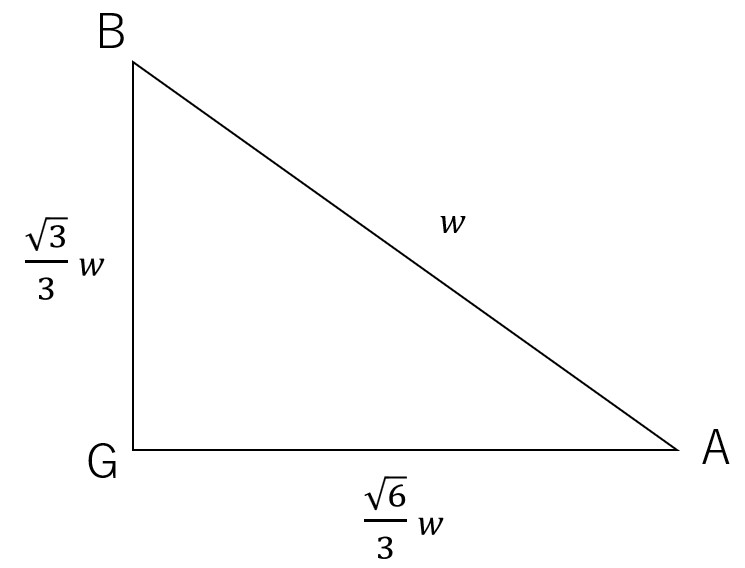
\includegraphics[width=6cm,keepaspectratio]{BGA.jpg}
    \caption{$\triangle{\rm{BGA}}$}
    \label{fig:bga}
  \end{center}
\end{minipage}
\end{center}
\end{figure}

\subsection{課題II-2}
一辺の長さを$w$とする正四面体の重心と原点$O$が重なるように正四面体を平行移動させ,$w$の値を調整することで,原点$O$を中心とする半径1の球に正四面体を内接させることができる.

平行移動後の$\triangle{\rm{BCD}}$の重心位置$G$と原点$O$の距離を$l$とし,$w$と$l$を求める.図\ref{fig:bga2}に示す$\triangle{\rm{BGA}}$と$\triangle{\rm{BGO}}$に三平方の定理を適用すると,以下の式が得られる.
\begin{displaymath}
\left\{
\begin{array}{l}
\left( \frac{\sqrt{3}}{3}w \right)^2 + (l + 1)^2 = w^2 \\
\left( \frac{\sqrt{3}}{3}w \right)^2 + l^2 = 1^2
\end{array}
\right.
\end{displaymath}

これを解くと,以下のようになる.
\begin{displaymath}
\left\{
\begin{array}{l}
w = \frac{2\sqrt{6}}{3} \\
l = \frac{1}{3}
\end{array}
\right.
\end{displaymath}
\begin{figure}[htbp]
\begin{center}
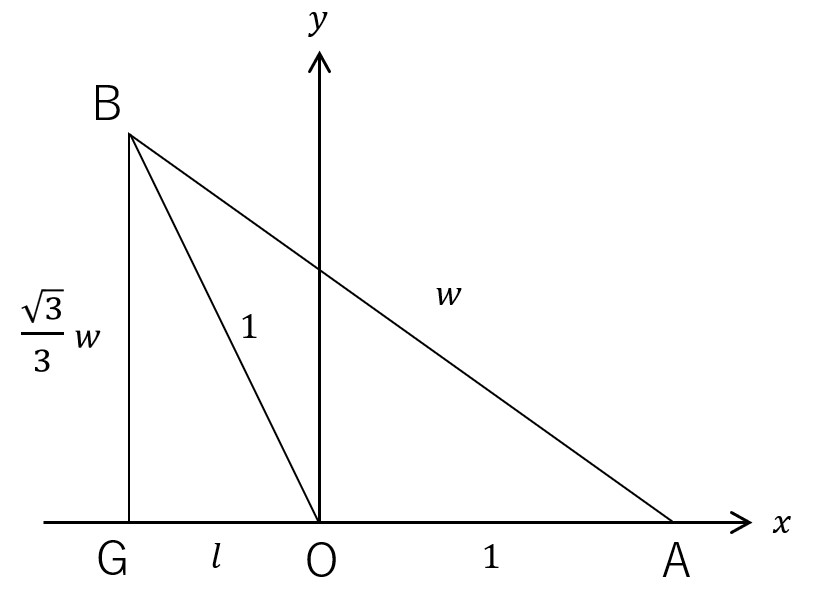
\includegraphics[height=4cm,keepaspectratio]{BGA2.jpg}
    \caption{平行移動後の$\triangle{\rm{BGA}}$}
    \label{fig:bga2}
\end{center}
\end{figure}

上記の値を課題II-1の結果に適用すると,正四面体の頂点がリスト14のように定まることがわかる.

\subsection{課題II-3}
ロボットアームを構成するプログラムの主要部をソースコード\ref{armtouroku}に示す.

\begin{lstlisting}[caption=ロボットアームの情報,label=armtouroku]
void init() {
    glClearColor(1.0, 1.0, 1.0, 1.0);
    myQuad = gluNewQuadric();

    glNewList(ID_B, GL_COMPILE);
    glColor3f(0.0, 0.0, 0.0);
    glPushMatrix();
    glRotated(90.0, 1.0, 0.0, 0.0);
    gluCylinder(myQuad, RADIUS_B, RADIUS_B, HEIGHT_B, 10, 2);
    glPopMatrix();
    glEndList();

    glNewList(ID_L, GL_COMPILE);
    glColor3f(0.0, 0.0, 1.0);
    glPushMatrix();
    glTranslated(0.0, 0.5 * HEIGHT_L, 0.0);
    glScalef(WIDTH_L, HEIGHT_L, WIDTH_L);
    glutWireCube(1.0);
    glPopMatrix();
    glEndList();

    glNewList(ID_U, GL_COMPILE);
    glColor3f(1.0, 0.0, 0.0);
    glPushMatrix();
    glTranslated(0.0, 0.5 * HEIGHT_U, 0.0);
    glScalef(WIDTH_U, HEIGHT_U, WIDTH_U);
    glutWireCube(1.0);
    glPopMatrix();
    glEndList();

}
\end{lstlisting}

次に,キーボードコールバック関数をソースコード\ref{armkeycall}に示す.
\begin{lstlisting}[caption=キーボードコールバック関数,label=armkeycall]
void keyin(unsigned char key, int x, int y) {
    switch (key) {
    case 'x':
        rotAng[0] += SPEED;
        glutPostRedisplay();
        break;

    case 'z':
        rotAng[0] -= SPEED;
        glutPostRedisplay();
        break;

    case 's':
        rotAng[1] += SPEED;
        glutPostRedisplay();
        break;

    case 'a':
        rotAng[1] -= SPEED;
        glutPostRedisplay();
        break;

    case 'w':
        rotAng[2] += SPEED;
        glutPostRedisplay();
        break;

    case 'q':
        rotAng[2] -= SPEED;
        glutPostRedisplay();
        break;

    default: break;
    }
}
\end{lstlisting}

特定のキーを入力すると,rotAngの値が変化し,ロボットアームを動かすことができるようになる.q,w,a,s,z,xで台座やロボットアームを動かす.キーボード配列で右側のキーが増加,左側のキーが現象をするようになっている.また,SPEEDの値を変化させることで台座の回転角や各関節の傾斜角の変化量を変えることができる.

\subsection{課題II-4}
実装したタイマコールバック関数をソースコード\ref{timercallbuck}に示す.
\begin{lstlisting}[caption=タイマコールバック関数,label=timercallbuck]
static void timer(int dummy) {
    glutTimerFunc(100, timer, 0);
    glMatrixMode(GL_MODELVIEW);

    rotAng[0] += 30;
    rotAng[1] += 10 * cos(time / 5);
    rotAng[2] += 100 * cos(time);
    time++;

    glutPostRedisplay();
}
\end{lstlisting}

台座に関しては2つの方向に動くと震えているように見えたため,一定方向に素早く回転するようにした.アームに関しては,2つの方向に動かした方がより踊っているように見えたため,三角関数を用いた.上のアームの動きは早くし,下のアームの動きは少しゆっくりにすることで,全力で踊っているように見せることができた.踊っているロボットアームを図\ref{fig:dance}に示す.
\begin{figure}[htbp]
\begin{center}
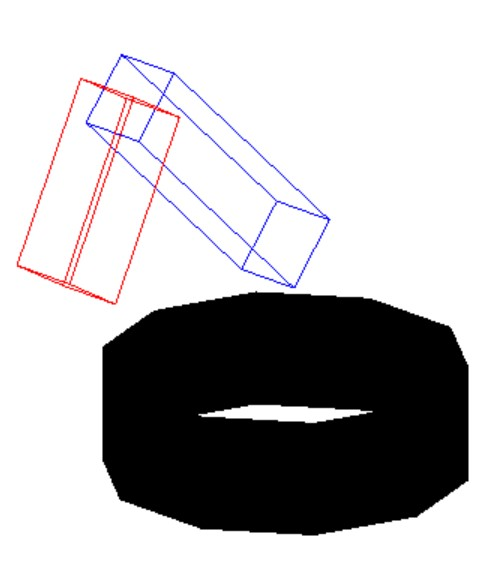
\includegraphics[height=4cm,keepaspectratio]{dance.jpg}
    \caption{踊っているロボットアーム}
    \label{fig:dance}
\end{center}
\end{figure}

\section{課題III}
\subsection{課題III-1}
2つのベクトルの外積は,その2つのベクトルが成す平面の法線ベクトルになる.$\overrightarrow{P_1 P_2}$,$\overrightarrow{P_2 P_3}$を2つのベクトルとし,$\triangle{P_1P_2P_3}$をベクトルの成す平面とすると,$\overrightarrow{P_1 P_2}\times\overrightarrow{P_2 P_3}$によって,$\triangle{P_1P_2P_3}$の単位法線ベクトルを全て求めることができる.

$\triangle{P_1P_2P_3}$の全ての単位法線ベクトルを$\overrightarrow{n}$とすると,以下のようになる.
$$
\overrightarrow{n} = \pm\frac{\overrightarrow{P_1 P_2}\times\overrightarrow{P_2 P_3}}{|\overrightarrow{P_1 P_2}\times\overrightarrow{P_2 P_3}|}
$$
\subsection{課題III-2}
空間中の任意の3点が与えられたとき,$\triangle{P_1P_2P_3}$の3点を反時計回りにたどる向きのベクトルから単位法線ベクトルを求めると,その単位法線ベクトルは面の表側を向く.これにより面の表裏を判別できる.
\subsection{課題III-3}
Phongモデルとは,物体の反射特性を数式で表現した最初のモデルである.Phongモデルでは,拡散反射成分は入射角の余弦と入射光の強さに比例するとされている.以下に式を示す.
\begin{eqnarray*}
I_d = I_i k_d \cos\alpha = I_i k_d (L・N)
\end{eqnarray*}

ここで,$I_d$は拡散反射光の強さ,$I_i$は入射光の強さ,$k_d$は拡散反射率,$\alpha$は入射角,$L$は光源方向ベクトル,$N$は表面法線ベクトルを示す.

また,Phongモデルは,鏡面反射光の強さは入射角の余弦の$n$乗と鏡面反射率に比例するとされている.以下に式を示す.
\begin{eqnarray*}
S = I_i W \cos^n\gamma
\end{eqnarray*}

ここで$S$は鏡面反射光の強さ,$n$はハイライトの特性,$\gamma$は光源の反射ベクトルと視線ベクトルのなす角を示す.また,厳密には鏡面反射率は光の波長によって異なるが,一定値$W$とされている.

そして,拡散,鏡面反射,環境光の3要素を考慮した場合の光の強さは次式のように表される.
\begin{eqnarray*}
I = k_d \cos\alpha + I_i W \cos^n \gamma + I_a k_a
\end{eqnarray*}

ここで,$I$は視点に入射する光の強さで,$I_a$は環境光の強さ,$k_a$は環境光定数を示している.

\subsection{課題III-4}
頂点の法線ベクトルは,重心からその頂点に向かう向きとなる.よって,原点を中心とする半径1の円に内接する正多面体の頂点の法線ベクトルは,その頂点の位置ベクトルと一致する.正四面体,正六面体,正八面体を描画するプログラムの主要部をソースコード\ref{seisimentai},\ref{seirokumentai},\ref{seihatimentai}にそれぞれ示す.

\begin{lstlisting}[caption=正四面体の描画,label=seisimentai]
GLdouble vP[4][3] = {
    {1.000, 0.000, 0.000},
    {-0.333, 0.943, 0.000},
    {-0.333, -0.471, 0.816},
    {-0.333, -0.471, -0.816}
};
int tP[4][3] = {
    {0, 1, 2},{0, 3, 1},
    {0, 2, 3},{1, 3, 2}
};

void display() {
    int i, j;
    glClear(GL_COLOR_BUFFER_BIT | GL_DEPTH_BUFFER_BIT);
    glMatrixMode(GL_MODELVIEW);
    glLoadIdentity();
    
    glBegin(GL_TRIANGLES);
    for (i = 0; i < 4; i++) {
        for (j = 0; j < 3; j++) {
            glNormal3dv(vP[tP[i][j]]);
            glVertex3dv(vP[tP[i][j]]);
        }
    }
    glEnd();
    glutSwapBuffers();
}
\end{lstlisting}
\begin{lstlisting}[caption=正六面体の描画,label=seirokumentai]
GLdouble vP[8][3] = {
    {-0.577,-0.577,0.577},{0.577,-0.577,0.577},
    {0.577,-0.577,-0.577},{-0.577,-0.577,-0.577},
    {-0.577,0.577,0.577}, {0.577,0.577,0.577},
    {0.577,0.577,-0.577}, {-0.577,0.577,-0.577}
};
int tP[6][4] = {
    {3,2,1,0},{0,1,5,4},{1,2,6,5},
    {4,5,6,7},{3,7,6,2},{0,4,7,3}
};

void display() {
    int i, j;
    glClear(GL_COLOR_BUFFER_BIT | GL_DEPTH_BUFFER_BIT);
    glMatrixMode(GL_MODELVIEW);
    glLoadIdentity();
    
    glBegin(GL_TRIANGLES);
    for (i = 0; i < 6; i++) {
        for (j = 0; j < 4; j++) {
            glNormal3dv(vP[tP[i][j]]);
            glVertex3dv(vP[tP[i][j]]);
        }
    }
    glEnd();
    glutSwapBuffers();
}
\end{lstlisting}
\begin{lstlisting}[caption=正八面体の描画,label=seihatimentai]
GLdouble vP[6][3] = {
    {1,0,0},{0,1,0},{0,0,1},
    {-1,0,0},{0,-1,0},{0,0,-1}
};
int tP[8][3] = {
    {0,1,2},{5,1,0},{3,1,5},{2,1,3},
    {2,4,0},{0,4,5},{5,4,3},{3,4,2}
};

void display() {
    int i, j;
    glClear(GL_COLOR_BUFFER_BIT | GL_DEPTH_BUFFER_BIT);
    glMatrixMode(GL_MODELVIEW);
    glLoadIdentity();
    
    glBegin(GL_TRIANGLES);
    for (i = 0; i < 8; i++) {
        for (j = 0; j < 3; j++) {
            glNormal3dv(vP[tP[i][j]]);
            glVertex3dv(vP[tP[i][j]]);
        }
    }
    glEnd();
    glutSwapBuffers();
}
\end{lstlisting}

\texttt{vP}に頂点の位置,\texttt{tP}にトポロジ情報を格納している.法線ベクトルの指定には,\texttt{vP}をそのまま利用している.

このプログラムを利用して描画した図形をそれぞれ図\ref{fig:4s},\ref{fig:6s},\ref{fig:8s}に示す.

\begin{figure}[htbp]
\begin{center}
\begin{minipage}[b]{0.45\textwidth}
  \begin{center}
    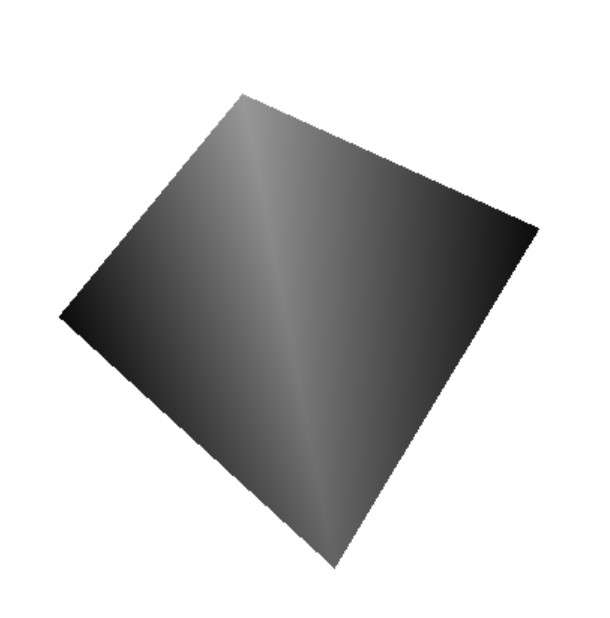
\includegraphics[width=4cm,keepaspectratio]{4s.jpg}
    \caption{正四面体}
    \label{fig:4s}
  \end{center}
\end{minipage}
\begin{minipage}[b]{0.45\textwidth}
  \begin{center}
    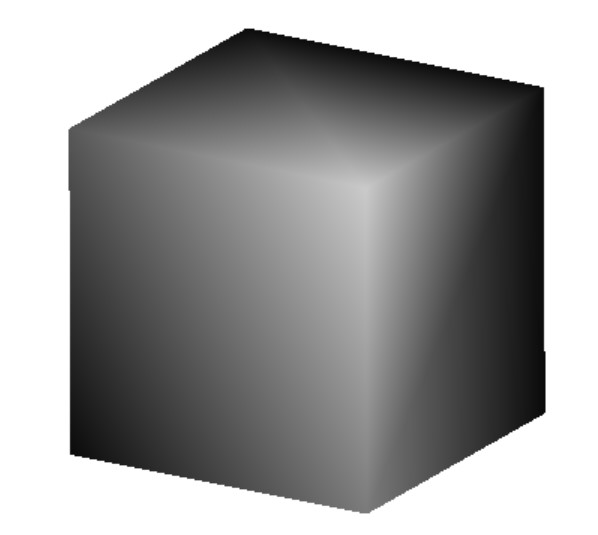
\includegraphics[width=4cm,keepaspectratio]{6s.jpg}
    \caption{正六面体}
    \label{fig:6s}
  \end{center}
\end{minipage}
\begin{minipage}[b]{0.45\textwidth}
  \begin{center}
    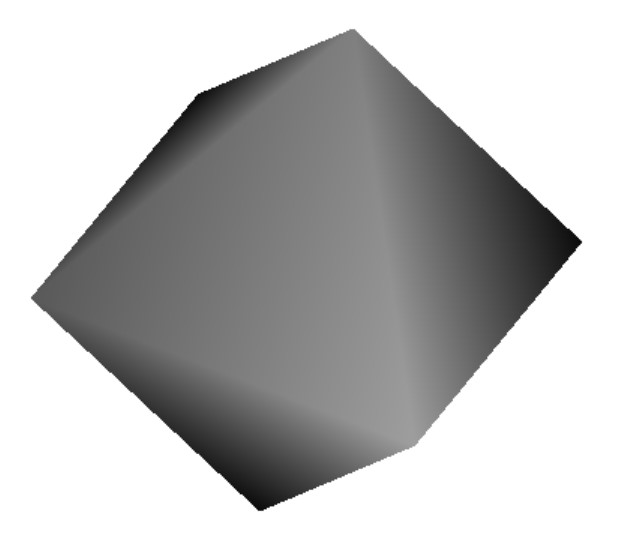
\includegraphics[width=4cm,keepaspectratio]{8s.jpg}
    \caption{正八面体}
    \label{fig:8s}
  \end{center}
\end{minipage}
\end{center}
\end{figure}



\subsection{課題III-5}
リスト27のロケットをアームロボットに変更した.各パーツの回転角度を格納するためのrotAngをグローバル変数として定義し,display関数内にはglRotatedを加えた.また,タイマーコールバック関数を用いて課題II-4のように踊って見えるようにした.変更したプログラムをソースコード\ref{real}に示す.
\begin{lstlisting}[caption=リスト27の変更部分,label=real]
GLdouble rotAng[3] = { 0 };

void display(void) {
	glClear(GL_COLOR_BUFFER_BIT | GL_DEPTH_BUFFER_BIT);
	glMatrixMode(GL_MODELVIEW);
	glLoadIdentity();
	gluLookAt(1.0, 1.0, 1.0, 0.0, 0.5, 0.0, 0.0, 1.0, 0.0);
	glRotated(rotAng[0], 0, 1, 0);
	glCallList(ID_B);
	glTranslatef(0.0, HEIGHT_B, 0.0);
	glRotated(rotAng[1], 0, 0, 1);
	glCallList(ID_L);
	glTranslatef(0.0, HEIGHT_L, 0.0);
	glRotated(rotAng[2], 0, 0, 1);
	glCallList(ID_U);
	glutSwapBuffers();
}

static void timer(int dummy) {
	glutTimerFunc(100, timer, 0);
	glMatrixMode(GL_MODELVIEW);

	rotAng[0] += 30;
	rotAng[1] += 10 * cos(time / 5);
	rotAng[2] += 100 * cos(time);
	time++;

	glutPostRedisplay();
}
\end{lstlisting}

踊っているロケットを図\ref{fig:rdance}に示す.

\begin{figure}[htbp]
\begin{center}
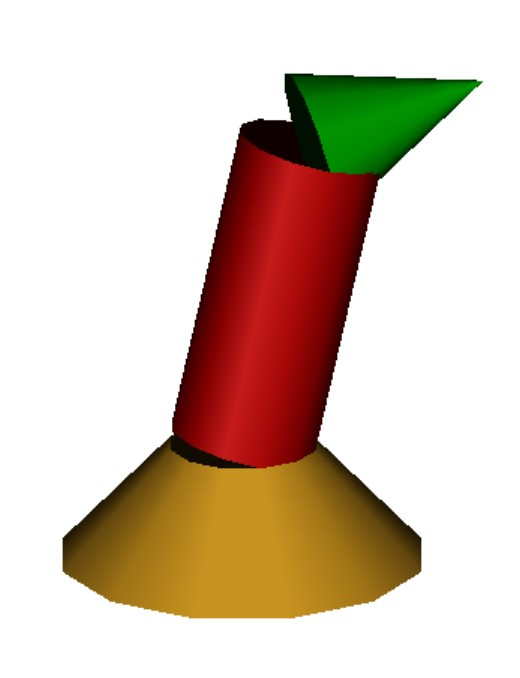
\includegraphics[height=4cm,keepaspectratio]{rdance.jpg}
    \caption{踊っているロケット}
    \label{fig:rdance}
\end{center}
\end{figure}

\section{感想}
これまで学習してきた内容に比べて難しく感じる箇所が多い科目ではあったが,楽しく学習することができた.進学先では使う機会が少なくなりそうではあるが,個人的に学習を進めていきたいと思う.

総合課題は学園祭の演劇と時期が近いため,時間を効率的に使って制作を進めていきたい.

\section{改善案}
全体的に改善するところはあまり思いつかなかった.細かい部分で挙げるとすれば,ワールド座標系とデバイス座標系の変換イメージの図をテキストにも載せてあると良いと思った.また,サポートページにあるスライドに音声があると聞き逃した場所などの復習ができて良いと思った.

\begin{thebibliography}{99}
\bibitem{1} https://tokoik.github.io/GLFWdraft.pdf
\bibitem{2} https://www.glfw.org/
\bibitem{3} https://forest.watch.impress.co.jp/article/1999/07/13/glui.html
\bibitem{4} https://www.dospara.co.jp/5info/cts\_str\_pc\_vulkan
\bibitem{5} https://www.khronos.org/opengles/
\bibitem{6} https://wgld.org/
\bibitem{7} https://docs.oracle.com/cd/E19957-01/806-4833/Make.html
\bibitem{8} https://eng-entrance.com/linux-command-grep
\bibitem{9} https://atmarkit.itmedia.co.jp/ait/articles/1606/14/news013.html
\bibitem{10} https://cmake.org/
\bibitem{1} https://subversion.apache.org/
\bibitem{1} https://git-scm.com/
\bibitem{1} http://ki-www.cvl.iis.u-tokyo.ac.jp/thesis/senior/inaguma.pdf
\bibitem{1} 柴田望洋,新・明解C言語,SBクリエイティブ株式会社,2014
\bibitem{6} 高橋章,R04-Ec5 プログラミング演習$\rm I\hspace{-.01em}I$テキスト
\end{thebibliography}

\end{document}


\begin{lstlisting}[caption=,label=]

\end{lstlisting}

